\documentclass[10pt]{article}
\usepackage[utf8]{inputenc}
\usepackage[T1]{fontenc}
\usepackage{amsmath}
\usepackage{amsfonts}
\usepackage{amssymb}
\usepackage[version=4]{mhchem}
\usepackage{stmaryrd}
\usepackage{graphicx}
\usepackage[export]{adjustbox}
\graphicspath{ {./images/} }
\usepackage{caption}

%New command to display footnote whose markers will always be hidden
\let\svthefootnote\thefootnote
\newcommand\blfootnotetext[1]{%
  \let\thefootnote\relax\footnote{#1}%
  \addtocounter{footnote}{-1}%
  \let\thefootnote\svthefootnote%
}

%Overriding the \footnotetext command to hide the marker if its value is `0`
\let\svfootnotetext\footnotetext
\renewcommand\footnotetext[2][?]{%
  \if\relax#1\relax%
    \ifnum\value{footnote}=0\blfootnotetext{#2}\else\svfootnotetext{#2}\fi%
  \else%
    \if?#1\ifnum\value{footnote}=0\blfootnotetext{#2}\else\svfootnotetext{#2}\fi%
    \else\svfootnotetext[#1]{#2}\fi%
  \fi
}

\begin{document}

\section*{12 Co-orbital satellites (50 Points)}
This question applies a method of determining the masses of two approximately co-orbital satellites developed by Dermott and Murray in 1981.\\
Suppose that two small satellites of masses $m_{1}$ and $m_{2}$ are approximately co-orbital (moving on very similar orbits) around a large central body of mass $M$, with $m_{1}, m_{2} \ll M$. At any instant, the orbits of the satellites may be approximated as circular Keplerian orbits with radii $r_{1}$ and $r_{2}$ respectively, although $r_{1}$ and $r_{2}$ will vary slightly over time due to the mutual gravitational interaction between the satellites.\\
Figure 4 depicts the shapes of the orbits in the rotating reference frame with zero angular momentum, centred on the central body. We denote by $\theta$ the angle $\measuredangle m_{1} M m_{2}$, while $R, x_{1}$, and $x_{2}$ denote the mean orbital radius and radial deviations of the satellites.\\
Throughout this problem, write all answers in an inertial reference frame.\\
Hint: $(1+x)^{\alpha} \approx 1+\alpha x$ for $\alpha x \ll 1$\\
First we will determine the value of $\frac{m_{1}}{m_{2}}$.\\
(a) Write down the angular momentum $L_{i}$ of the satellite with mass $m_{i}$ when its circular orbit has radius $r_{i}$.\\
(b) The satiletes total angular momentum $L_{1}+L_{2}$ is conserved. Let $x_{1}, x_{2} \ll R$ be the distances as shown in Figure 4. Find a simple relation between the ratios $\frac{m_{1}}{m_{2}}$ and $\frac{x_{1}}{x_{2}}$.

Now, we will try and determine the value of $m_{1}+m_{2}$. For next parts, we will use the actual barycenter of the system, which may not be exactly at the center of the planet.\\
(c) The individual angular momenta of the satellites $m_{1}$ and $m_{2}$ will vary over time due to their gravitational interactions. Show that the rate of change of the angular momentum of the second satellite is given by


\begin{equation*}
\frac{\Delta L_{2}}{\Delta t} \approx-\frac{G m_{1} m_{2}}{R} h(\theta) \quad \text { where } \quad h(\theta)=\left[\frac{\cos \left(\frac{\theta}{2}\right)}{4 \sin ^{2}\left(\frac{\theta}{2}\right)}-\sin \theta\right] \tag{18pt}
\end{equation*}


(d) Show that $s=r_{2}-r_{1}$ satisfies


\begin{equation*}
\frac{\Delta s}{\Delta t} \approx-2 \sqrt{\frac{G}{M R}}\left(m_{1}+m_{2}\right) h(\theta) \tag{8pt}
\end{equation*}


(e) For the angle $\theta=\measuredangle m_{1} M m_{2}$ as indicated on Figure 4, find an expression for $\frac{\Delta \theta}{\Delta t}$\\
(f) Using the results above, find the relation between $\Delta s$ and $\Delta \theta$.\\
(g) After integrating the expression above, we will obtain the result,

$$
\bar{x}^{2} \approx \frac{4 R^{2}}{3} \frac{m_{1}+m_{2}}{M}\left(\frac{1}{\sin \left(\frac{\theta_{\min }}{2}\right)}-2 \cos \theta_{\min }-3\right)
$$

where $\bar{x}=\frac{x_{1}+x_{2}}{2}$.\\
Epimetheus ( $m_{1}$ ) and Janus ( $m_{2}$ ) are two approximately co-orbital moons of Saturn. Detailed observations of their orbits have been performed by the Voyager 1 and Cassini spacecraft, which found that $R=150000 \mathrm{~km}, x_{1}=76 \mathrm{~km}$ and $x_{2}=21 \mathrm{~km}$. The minimum distance between Janus and Epimetheus is 13000 km . The mass of Saturn is known to be $5.7 \times 10^{26} \mathrm{~kg}$. Estimate the masses of Epimetheus and Janus.

\begin{figure}[h]
\begin{center}
  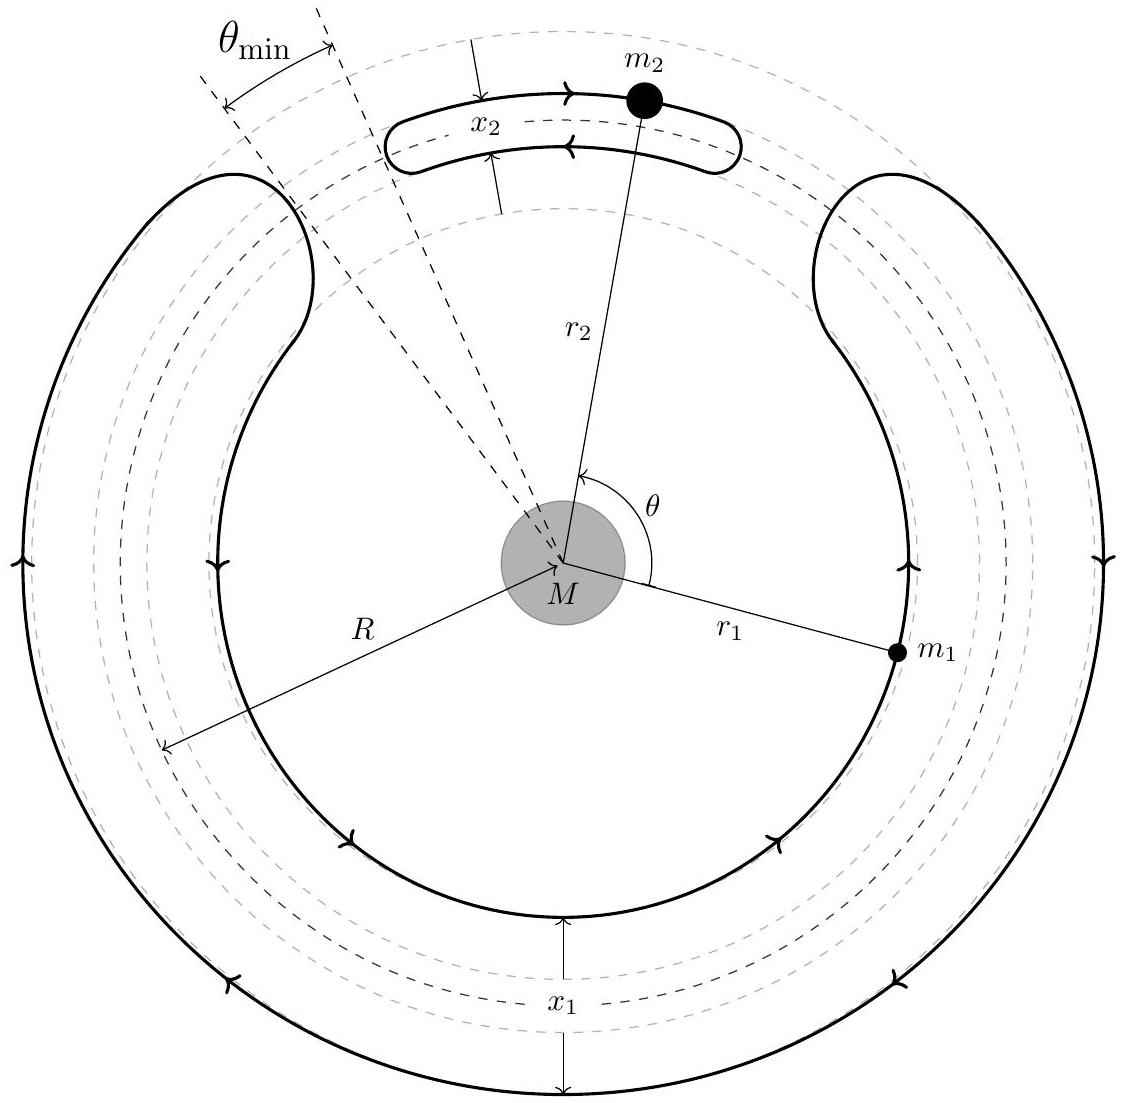
\includegraphics[width=\textwidth]{2025_09_11_6312450c103d6a7e5736g-09}
\captionsetup{labelformat=empty}
\caption{Figure 4: This figure schematically depicts the shapes of the orbits in the rotating reference frame, selected such that in this frame the total angular momentum of the two satellites is zero.}
\end{center}
\end{figure}


\end{document}